\documentclass[12pt]{article}
\usepackage{amssymb, amsmath, amsfonts, bm, graphicx, geometry}
\usepackage{tabularx, booktabs, float, enumitem, multicol, mathtools,caption}
\geometry{margin=1in}

\title{}
\date{}
\author{}

% Uppercase Volume with thicker, higher line
\newcommand{\vol}{\mathord{\text{\ooalign{\hidewidth $V$\hidewidth\cr\kern-0.5pt\raisebox{0.8ex}{\rule[0pt]{1em}{0.5pt}}}}}}

% Lowercase Volume with built-in shifts
\newcommand{\svol}{%
  \mathord{\text{\ooalign{%
    \hspace{0.1em}$v$\cr         % built-in horizontal shift of 'v'
    \hspace{-0.02em}\rule[0.6ex]{0.8em}{0.5pt} % built-in horizontal shift of the bar, vertical raise, length, thickness
  }}}%
}
\begin{document}

\begin{center}
{\LARGE ESC-330 Engineering Thermodynamics Notes\par}
\end{center}
The key question in thermodynamics is: \textit{How can we use energy to do work?} Accordingly, we will be looking at the ways in which energy is stored, transformed, and transferred, as constrained by the laws of thermodynamics (conservation of energy and the increase of entropy), as well as the accompanying changes in the state of matter. To begin, we will define some key concepts such as systems, states, processes, and properties which are the frame through which we will analyze thermodynamic processes.\\\\
The \textbf{First Law of Thermodynamics} states that energy is conserved: energy can be transferred or transformed, but the total energy of an isolated system remains constant.\\\\
The \textbf{Second Law of Thermodynamics} states that while energy is conserved, real processes are irreversible and occur in a preferred direction, leading to an increase in the entropy of an isolated system. This increase in entropy reduces the maximum amount of work that can be extracted from energy.\\\\
Entropy is a thermodynamic property that quantifies irreversibility and constrains the availability of energy to perform work.\\\\
Also note that thermodynamics is a science that emerged in the 1800s, around the same time as the development of the steam engine, before modern chemistry and physics were fully established. As a result, it is primarily an observational and experimental science, focusing on the macroscopic properties and behavior of matter rather than the microscopic details of atoms and molecules.
\vspace{1em}
\noindent\hrule
\vspace{1em}
\begin{center}
{\LARGE Chapter 1: Introduction and Basic Concepts\par}
\end{center}
\section*{Systems and Control Volumes}
In thermodynamics, we begin every problem by defining a \textbf{system} which is a quantity of matter or a region in space chosen for study. The \textbf{surroundings} are everything outside the system, and the \textbf{boundary} is the real or imaginary surface that separates the system from its surroundings. \\\\
When defining a system, we are mostly interested in regions that contain \textit{mass} since fundamentally, mass is the carrier of energy. Therefore, we specify two types of systems: closed systems and open systems.\\\\
In a \textbf{closed system} (or \textit{control mass}), a fixed amount of matter is enclosed, and no mass crosses the boundary. In an \textbf{open system} (or \textit{control volume}), a specified region in space is enclosed, and mass may flow across the boundary. For both closed and open systems, energy may cross the boundary in the form of heat or work.\\\\
Because a closed system does not permit mass transfer, energy transfer is limited to heat and boundary work; mechanical energy associated with mass flow (kinetic, potential, and flow energy) cannot cross the boundary. In contrast, an open system allows mass transfer, enabling energy to be carried across the boundary in the form of kinetic, potential, and flow energy, in addition to heat transfer and work.\\\\
\underline{Note:} \textbf{Flow energy} is the pressure work per unit mass associated with mass flow, it describes the energy needed to push mass into or out of a control volume against pressure (like in pumps). 
\[\boxed{\text{Flow Energy} = P\svol}\]
Note that while pressure isn't a form of energy, when a pressure force acts on a fluid through a distance, it does \textit{flow work}. In fact the units of pressure is energy per unit volume: Pa = N/m$^2$ = N$\cdot$m/m$^3$ = J/m$^3$. In this case, we used $\svol$ which is the specific volume (volume per unit mass).\\\\
A \textbf{isolated system} is a special type of closed system that does not exchange either mass or energy with its surroundings.\\\\
\underline{Ex}: Piston–cylinder (closed sys): gas does work by moving the piston and heat can cross the walls. Nozzle (open sys): fluid carries energy as it flows through the system.
\begin{center}
    \includegraphics[width=0.3\textwidth]{Piston.png}
    \hspace{0.05\textwidth}
    \includegraphics[width=0.3\textwidth]{Nozzle.png}
\end{center}
\textbf{Control surfaces} are the boundaries of control volumes. They may be real or imaginary, fixed or moving.
\section*{Properties}
In classical thermodynamics, we focus on macroscopic, measurable characteristics of a system, ignoring microscopic behavior like molecular interactions. A \textbf{property} is thus a macroscopic quantity that can be measured at a single instant in time. Properties exclude quantities such as energy or work, which describe the system’s interactions with its surroundings rather than the system itself.\\\\
We define properties as extensive and intensive. \textbf{Extensive properties} depend on the size or mass of the system, while \textbf{intensive properties} do not. By normalizing an extensive property by mass, we obtain a \textbf{specific property}, which is intensive. Intensive and specific properties are particularly useful for describing a system’s state, since they are independent of the amount of matter present.
\begin{center}
\begin{tabular}{|l|l|}
\hline
\textbf{Extensive Properties} & \textbf{Intensive Properties} \\
\hline
Temperature: $T$ & $T$ \\
Pressure: $P$ & $P$ \\
Volume: $\vol$ & Specific Volume: $\svol = \vol / m$ \\
Internal Energy: $U$ & Specific Internal Energy: $u = U / m$ \\
Entropy: $S$ & Specific Entropy: $s = S / m$ \\
\hline
\end{tabular}
\end{center}
\underline{Note:} Internal energy $U$ and entropy $S$ are examples of extensive properties that cannot be measured directly. However, they do have a definite value at any given state, found using changes in these properties from a reference state.
\[\Delta U = Q - W\]  
\[\Delta S = \int \frac{\delta Q_\mathrm{rev}}{T}\]  
where $Q$ is the heat added to the system and $W$ is the work done by the system, and $\delta Q_\mathrm{rev}$ is the infinitesimal heat transfer in a reversible process. Internal energy is then the energy contained, well, within the system since $Q$ and $W$ represent energy transfer across the boundary.\\\\
\textbf{Density and Specific Gravity}
\[\rho = \frac{m}{\vol}\quad \text{(density)}\]
\[\svol = \frac{\vol}{m} = \frac{1}{\rho} \quad \text{(specific volume)}\]
\textbf{Specific gravity} is defined as a relative density compared to water (at 4$^\circ$C) where $\rho_{water} = 1000\,\text{kg/m}^3$:
\[\boxed{SG = \frac{\rho_{fluid}}{\rho_{water}} \implies \rho_{fluid} = SG \cdot \rho_{water}}\]
\textbf{Specific Weight}
\[\gamma_s = \rho g \quad \text{(specific weight)}\]
Thus hydrostatic pressure can be written as $P = \rho gh=\gamma_s h$
\newpage
\section*{States and Equilibrium}
Now that we have defined properties, we can define the \textbf{state} of a system as the condition of the system described by its properties. The state can be visualized as a single point in a three-dimensional plot of pressure, temperature, and specific volume, with the properties serving as the coordinates of that point. The plot below shows a $P$–\;\,$\svol$–$T$ surface for a substance that expands upon freezing (like water). For a simple compressible system, specifying any two independent properties (such as $P$ and $T$) uniquely determines the third property ($\;\svol$) on the surface, this is known as the \textbf{state postulate}.
\vspace{-1em}
\begin{center}
    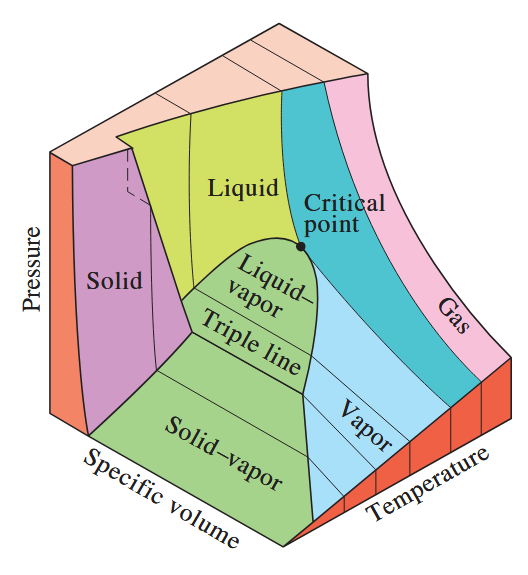
\includegraphics[width=0.4\textwidth]{State.png}
\end{center}\vspace{-1em}
\underline{Note:} A simple compressible system is one where electrical, magnetic, gravitational, motion, and surface tension effects are negligible. If any of these effects are significant, an extra property must be specified for each.\\\\
\textbf{Ideal Gas Equation of State}\\
A direct application of the state postulate is the ideal gas law, which defines the relationship between these three properties for an ideal gas, so that specifying any two properties automatically determines the third. The \textit{most general form} of the ideal gas law is:
\[\boxed{P \, \svol = R \, T, \quad
R = \frac{\bar{R}}{M} \quad \text{(specific gas constant, kJ/kg·K)}} \]
Where:
\begin{itemize}[label=\textbullet]
    \item $P$ = \textit{absolute} pressure (Pa)
    \item $\svol$ = specific volume (m$^3$/kg), where $\svol = \vol/m$
    \item $T$ = \textit{absolute} temperature (K)
    \item $M$ = molar mass of the gas (kg/mol)
\end{itemize}
and $\bar{R}$ is the universal gas constant:
\[\bar{R} = \begin{cases} 
8.31447 \text{ kJ/kmol} \cdot \text{K} \\
8.31447 \text{ kPa} \cdot \text{m}^3/\text{kmol} \cdot \text{K} \\
0.0831447 \text{ bar} \cdot \text{m}^3/\text{kmol} \cdot \text{K} \\
1.98588 \text{ Btu/lbmol} \cdot \text{R} \\
10.7316 \text{ psia} \cdot \text{ft}^3/\text{lbmol} \cdot \text{R} \\
1545.37 \text{ ft} \cdot \text{lbf/lbmol} \cdot \text{R}
\end{cases} \quad \text{(universal gas constant)}\]
In table A-2 the specific gas constant $R$ is given for various gases, so we do not need to calculate it using the molar mass $M$ and the universal gas constant $\bar{R}$. Additionally, if we multiply both sides of the ideal gas law by mass $m$, we can express it in terms of volume $\vol$ instead of specific volume $\svol$:
\[\boxed{P \, \vol = m R T}\]
Additionally, classical thermodynamics assumes that states are always in \textbf{equilibrium} and that processes occur in \textbf{quasi-equilibrium}, meaning the system remains balanced and changes happen slowly enough for it to adjust and maintain equilibrium throughout, and properties are well-defined. Below are some types of equilibrium that can exist in a system:
\begin{itemize}
\item \textbf{Thermal equilibrium} occurs when the temperature is uniform throughout the system.
\item \textbf{Mechanical equilibrium} occurs when there are no unbalanced forces within the system or with its surroundings, meaning pressure does not change at any point over time.
\item \textbf{Phase equilibrium} occurs when the different phases of a system (solid, liquid, gas) remain constant with no mass transfer.
\item \textbf{Chemical equilibrium} occurs when the chemical composition of the system does not change over time, with no reactions taking place.
\end{itemize}
\newpage
\section*{Pressure}
Pressure is a fundamental property in thermodynamics, defined as the normal force per unit area exerted by a fluid on a surface. 
\[P=F/A\]
\[P = \rho g h\quad \text{(hydrostatic pressure)}\]
When measuring pressure, we must specify the reference point. \textbf{Absolute pressure} is measured relative to a perfect vacuum, while \textbf{gauge pressure} is measured relative to atmospheric pressure. The relationship between them is:
\[\boxed{P_{\text{gauge}} = P_{\text{absolute}} - P_{\text{atmospheric}}}\]
\[\boxed{P_{\text{vacuum}} = P_{\text{atmospheric}} - P_{\text{absolute}}}\]
\underline{Note:} Generally, gauge pressures already account for atmospheric pressure, and thus reads zero when open to the atmosphere. This fact allows us to ignore atmospheric pressure when a problem involves only gauge pressures, since it will cancel out in the calculations.
\begin{center}
    \includegraphics[width=0.7\textwidth]{Gauge pressure.png}
\end{center}
\newpage\noindent
Below are some ways to calculate pressure:
\begin{itemize}
\item \textbf{Hydrostatic Pressure}\\
\begin{minipage}[t]{0.6\textwidth} \vspace{0pt}
This is probably the simplest way to calculate pressure, it is the pressure exerted by a fluid at rest due to the weight of the fluid above it. It can be calculated using the formula:
\[P = \rho g h\]
If we are finding absolute pressure, we need to add atmospheric pressure to this value: $P_{\text{absolute}} = P_{\text{atmo}} + \rho g h$. Gauge pressure ignores atmospheric pressure, so it is simply $P_{\text{gauge}} = \rho g h$.\\\\
\underline{Note:} If density is equal (ie. the fluid is continuous) then the pressure at equal depths are equal, regardless of the shape of the container, this will be used for Pascal's law.\\\\
\textbf{Pascal's Law} states that the pressure applied to a confined fluid increases the pressure throughout the fluid by the same amount. Therefore, in the hydraulic jack, Pascal's law allows a small force applied to the smaller piston to be transformed into a larger force on the larger piston, enabling us to lift heavy objects with less effort.
\[P_1=P_2 \quad \implies \quad \frac{F_1}{A_1} = \frac{F_2}{A_2} \quad \implies \frac{F_2}{F_1} = \frac{A_2}{A_1}\]
\end{minipage}
\hfill
\begin{minipage}[t]{0.4\textwidth} \vspace{0pt}
\centering
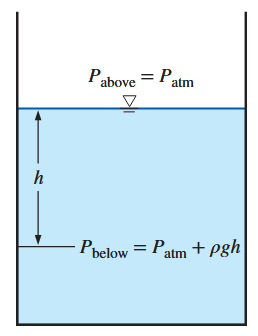
\includegraphics[width=\textwidth]{Hydrostatic.png}
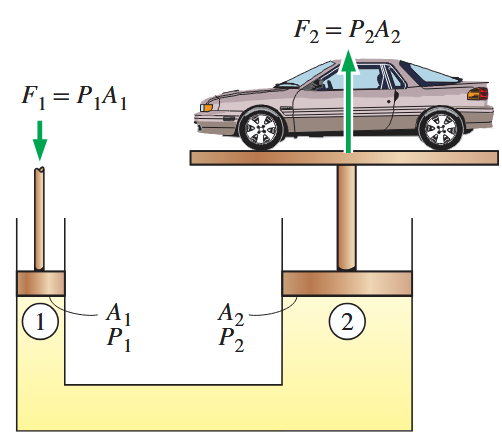
\includegraphics[width=\textwidth]{Pascal.png}
\end{minipage}
\newpage
\item \textbf{The Barometer}\\
\begin{minipage}[t]{0.6\textwidth} \vspace{0pt}
In the barometer, we apply the hydrostatic pressure formula to find the atmospheric pressure in terms of the height of mercury within the column $h$. From Pascal's law, the pressure at point B is equal to the atmospheric pressure (equal elevation), so we can write the force balance at B:
\[\sum F =0 \quad \implies \quad P_{\text{atm}} = \rho g h\]
Pressure at point C is approximately zero since there is only mercury vapor above it.
\end{minipage}
\hfill
\begin{minipage}[t]{0.4\textwidth} \vspace{0pt}
\centering
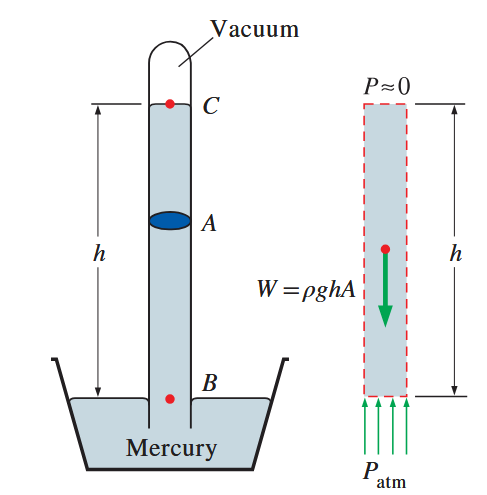
\includegraphics[width=\textwidth]{Barometer.png}
\end{minipage}
\item \textbf{The Manometer}\\
The manometer is a device that measures pressure differences, and thus can measure a pressure relative to atmospheric pressure (gauge pressure) or a pressure relative to a vacuum (absolute pressure). We will build the intuition for how to solve manometer problems by following the steps below:
\begin{itemize}
    \item \textbf{Basic Single Fluid Manometer:}\\
\begin{minipage}[t]{0.6\textwidth} \vspace{0pt}
The pressure in a fluid does not change with horizontal position (equal depth), so the pressure at points 1 and 2 are equal:
    \[P_1 = P_2\]
    Where we use the hydrostatic pressure formula to express the pressures at points 1 and 2:
    \[P_1 = P_{gas}, \quad P_2 = P_{atm} + \rho g h\]
\end{minipage}
\hfill
\begin{minipage}[t]{0.4\textwidth} \vspace{0pt}
\centering
        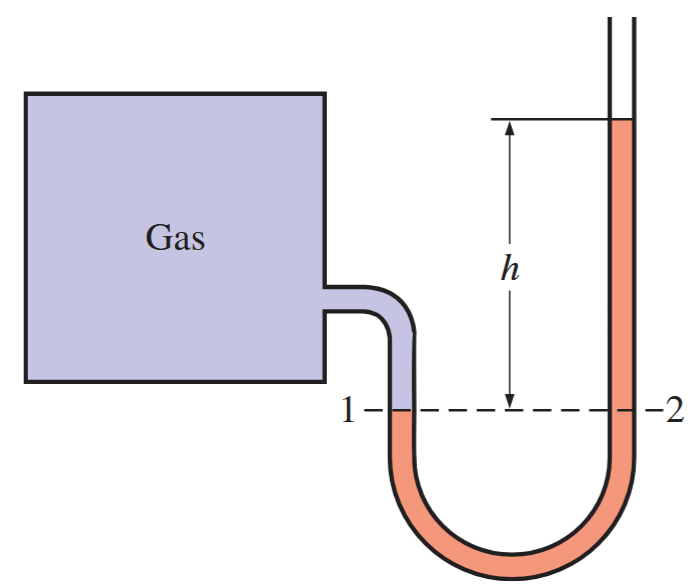
\includegraphics[width=\textwidth]{Manometer.png}
\end{minipage}
\newpage
    \item \textbf{Pressure with Multiple Layers of Fluid:}\\
\begin{minipage}[t]{0.6\textwidth} \vspace{0pt}
We use the following rules to find the pressure at different points in a fluid with multiple layers:
    \begin{enumerate}
        \item The pressure change across a fluid layer is given by the hydrostatic pressure formula: $\Delta P = \rho g h$
        \item Pressure increases downward (+) and decreases upward (-).
        \item The pressure at points of equal depth in a fluid are equal (Pascal's Principle).
    \end{enumerate}
    Ex: At point 1 in the figure, $P_1 = P_{atm}+\rho_1g h_1+\rho_2 g h_2 + \rho_3 g h_3$
\end{minipage}
\hfill
\begin{minipage}[t]{0.4\textwidth} \vspace{0pt}
\centering
        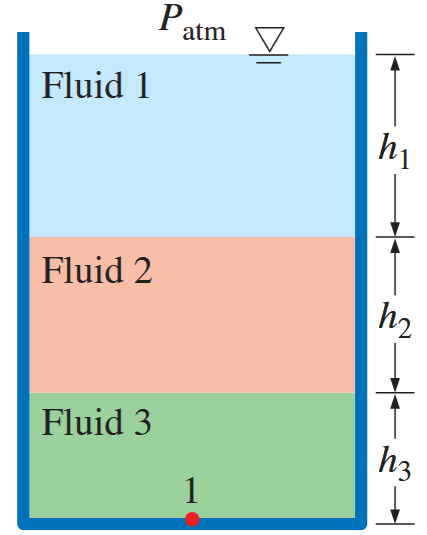
\includegraphics[width=\textwidth]{Stacked Fluid.png}
\end{minipage}
\item \textbf{Multi-fluid Manometer:}\\
\begin{enumerate}
    \item Begin at a known pressure point (gauge or atmospheric pressure) and follow the fluid layers to the unknown pressure point.
    \item Sign convention: add when going down, subtract when going up.
    \item \textbf{Horizontal jump:} We can "jump" horizontally across bends in the tube if both sides of the jump are within the \textbf{same continuous fluid}. This is because pressure is identical at the same horizontal level within a single static fluid. \textit{Any pressure decrease from moving upward is perfectly balanced by an equal pressure increase when moving back down to that same level on the other side.}
    \item The pressure at each end of the manometer equals the total pressure obtained by summing the contributions of all fluid columns along the vertical path.
\end{enumerate}   
\end{itemize}
\end{itemize}
\newpage\noindent
\underline{Ex: 1-110}\\
\begin{minipage}[t]{0.6\textwidth} \vspace{0pt}
\centering
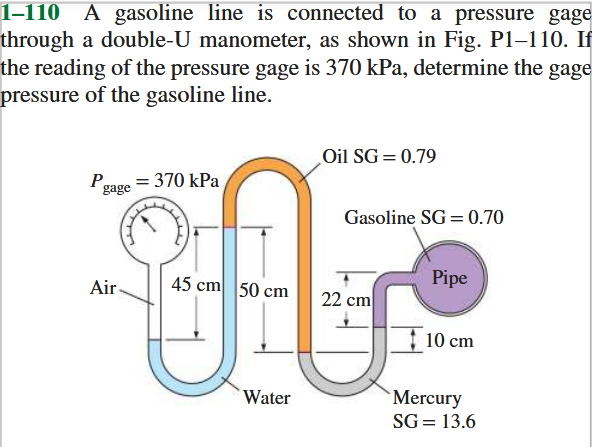
\includegraphics[width=\textwidth]{1-110.png}
\end{minipage}
\hfill
\begin{minipage}[t]{0.4\textwidth} \vspace{0pt}
Given:
\begin{itemize}
    \item $P_{gauge} = 370\,\text{kPa}$
    \item Specific gravities
    \begin{itemize}
        \item Oil: $SG_{oil} = 0.79$
        \item Mercury: $SG_{Hg} = 13.6$
        \item Gasoline: $SG_{gas} = 0.70$
    \end{itemize}
    \item Height differences:
    \begin{itemize}
        \item $h_{water} = 45\,\text{cm}$
        \item $h_{oil} = 50\,\text{cm}$
        \item $h_{Hg} = 10\,\text{cm}$
        \item $h_{gas} = 22\,\text{cm}$
    \end{itemize}
\end{itemize}
Find: 
\begin{itemize}
    \item Gauge pressure of gas line.
\end{itemize}
\end{minipage}\\\\\\
Therefore:
\[P_{gauge} - \rho_{water}gh_{water} + \rho_{oil}gh_{oil} - \rho_{Hg}gh_{Hg} - \rho_{gas}gh_{gas} = P_{gas}\]
\[\implies P_{gas} = P_{gauge} + \rho_{water}g(-h_{water} + SG_{oil}h_{oil} - SG_{Hg}h_{Hg} - SG_{gas}h_{gas})\]
Plugging in the values:
\[P_{gas} = [370\,\text{kPa}]+[1000\,\text{kg/m}^3][9.81\,\text{m/s}^2]\bigg(-[0.45\,\text{m}] + [0.79][0.5\,\text{m}] - [13.6][0.1\,\text{m}] - [0.70][0.22\,\text{m}]\bigg)\]
\[P_{gas} = [370\,\text{kPa}]-
\left[15391.89\,\frac{kg}{m\cdot s^2}\right]
\left[\frac{N}{kg \cdot m/s^2}\right]
\left[\frac{Pa}{N/m^2}\right]\]
\[= [370\,\text{kPa}]-
[15.391\,\text{kPa}] = 354.609\,\text{kPa} \approx \boxed{354.6\,\text{kPa}}\]
\section*{Temperature and Zeroth Law of Thermodynamics}
Before introducing temperature, we first define the \textbf{Zeroth Law of Thermodynamics}: if two systems are each in thermal equilibrium with a third system, they are in thermal equilibrium with each other. Replacing the third system with a \textit{thermometer} allows us to define temperature as a property that is the same for any two systems in thermal equilibrium.\newpage\noindent
\textbf{Temperature Conversions}
\begin{itemize}[label=\textbullet]
    \item Absolute temperature conversions
    \begin{itemize}[label=\textopenbullet]
        \item $T_{K} = T_{^\circ C} + 273.15$
        \item $T_{^\circ R} = T_{^\circ F} + 459.67$
        \item $T_{^\circ F} = \frac{9}{5}T_{^\circ C} + 32$
        \item $T_{^\circ R} = \frac{9}{5}T_{K}$
    \end{itemize}
    \item Temperature difference conversions
    \begin{itemize}[label=\textopenbullet]
        \item $\Delta K = \Delta ^\circ C$
        \item $\Delta ^\circ R = \Delta ^\circ F$
        \item $\Delta ^\circ F = \frac{9}{5}\Delta ^\circ C$
        \item $\Delta ^\circ R = \frac{9}{5}\Delta K$
    \end{itemize}
\end{itemize}
\underline{Note:} Fahrenheit and Celsius are relative temperature scales (based on the freezing/boiling points of water), while Rankine and Kelvin are absolute temperature scales (starting at absolute zero).
\section*{Processes}
\begin{minipage}[t]{0.6\textwidth} \vspace{0pt}
A \textbf{process} is a transformation that takes a system from one state to another, during which its properties change. The process can be represented by a \textbf{path}, which is the sequence of states the system passes through. The path is important because it determines the work and heat transfer, which depend on how the system moves between states rather than the states themselves.\\\\
\textbf{Types of Processes}
\begin{itemize}
    \item \textbf{Isobaric process}: constant pressure
    \item \textbf{Isochoric process}: constant volume 
    \item \textbf{Isothermal process}: constant temperature 
    \item \textbf{Adiabatic process}: no heat transfer
\end{itemize}
\end{minipage}
\hfill
\begin{minipage}[t]{0.4\textwidth} \vspace{0pt}
\centering
\includegraphics[width=\textwidth]{Process.png}
\end{minipage}
\vspace{1em}
\noindent\hrule
\vspace{1em}
\newpage
\begin{center}
{\LARGE Chapter 2: Energy, Energy Transfer, and General Energy Analysis\par}
\end{center}
In Chapter 2, we apply the First Law of Thermodynamics, the principle of conservation of energy, to the analysis of energy transfer in systems. Beyond tracking how much energy is transferred, we also focus on the \textit{rate} at which energy is transferred, known as power or the rate of work being done. In this chapter, we mostly focus on the energy transfer through the mechanism of work and heat separately on systems.
\section*{Forms of Energy and Energy Transfer}
As always, energy is the capacity to do work, the total energy of a system consisting of internal energy, kinetic energy, and potential energy is:
\[E = U + KE + PE = U + \frac{1}{2}mv^2 + mgh\]
or in specific form (per unit mass):
\[e = u + \frac{1}{2}v^2 + gh\]
As mentioned before, internal energy is the energy contained within the system, while kinetic and potential energy are forms of mechanical energy associated with the motion and position of the system.\\\\
\textbf{Mechanisms of Energy Transfer}
\begin{enumerate}
    \item \textbf{Heat Transfer} $Q$:\\
    Heat transfer \textit{to} a system increases its internal energy while heat transfer \textit{from} a system decreases its internal energy. Heat transfer can occur through three modes: conduction, convection, and radiation.
    \item \textbf{Work Transfer} $W$:\\
    Work is a common form of energy transfer and occurs when energy crosses a system boundary by means other than heat (temperature difference) or mass flow. It is associated with a force acting through a distance by mechanical means. Work can be done on a system, increasing its energy, or by a system, decreasing its energy.
    \item \textbf{Mass Flow} $\dot{m}$:\\
    Mass flow is a form of energy transfer that occurs in control volumes. As mass enters the system, it increases the system's energy because mass carries energy with it. Likewise, as mass leaves the system, it decreases the system's energy.
\end{enumerate}
\textbf{Closed Systems}\\
For closed systems where $\Delta KE = \Delta PE = 0$ are referred to as \textbf{stationary systems}. In a stationary system, energy transfer can occur only through heat and work, so the change in total energy is equal to the change in internal energy:
\[\Delta E = \Delta U\]
\[\boxed{\Delta U = Q - W}\]
\textbf{Open Systems}\\
For open systems (control volumes), mass can flow across the boundary, carrying energy with it. Most open systems involve fluid flow so it is easier to express energy flow associated with fluid flow in terms of rates.\\\\
We define the \textbf{mass flow rate} as the amount of mass flowing through a cross-section per unit time, it is related to the volumetric flow rate $\dot{\vol}$ by:
\[\boxed{\dot{m} = \rho \,\dot{\vol} = \rho A_c V_{\text{avg}} \quad [\text{kg/s}]}\]
Where $A_c$ is the cross-sectional area and $V_{\text{avg}}$ is the average velocity of the fluid normal to the cross-section.\\\\
Thus, the energy flow rate associated with fluid flowing at a rate of $\dot{m}$ is:
\[\dot{E} = \dot{m} e \quad \text{[J/s]}\]
The mechanical energy flow rate associated with fluid flow is the sum of flow, kinetic, and potential energy:
\[\boxed{e_{\text{mech}} = \frac{P}{\rho} + \frac{1}{2}v^2 + gz}\]
\section*{Energy Transfer by Work}
The most general definition of work is the energy transfer that occurs when a force acts through a distance. 
\[W = \int_{1}^{2} F \cdot dx\]
Here are some other types of work:
\begin{itemize}
    \item \textbf{Electrical work}\\
We know that the power associated with electrical work across a load of resistance $R$ is given by:
\[\dot{W}_{\text{elec}} = VI = RI^2 = \frac{V^2}{R}\]
Where $I$ is the current and $V$ is the voltage across the load. Thus, the work done over time $\Delta t$ when both $V$ and $I$ are constant is:
\[W_{\text{elec}} = \dot{W}_{\text{elec}} \Delta t = VI \Delta t\]
    \item \textbf{Shaft work}\\
\begin{minipage}[t]{0.6\textwidth} \vspace{0pt}
Where $n$ is the number of revolutions, $\dot{n}$ is the rate of revolutions, and $F$ is a constant force acting $r$ away:
\[W_{\text{shaft}} = F\Delta s = \left(\frac{T}{r}\right) (2\pi rn) = 2\pi nT\]
The power associated with shaft work is:
\[\dot{W}_{\text{shaft}} = 2\pi \dot{n} T\]
\end{minipage}
\hfill
\begin{minipage}[t]{0.4\textwidth} \vspace{0pt}
\centering
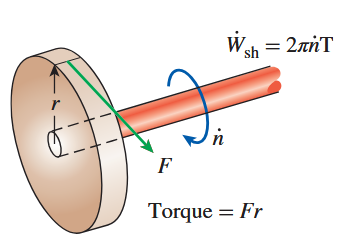
\includegraphics[width=\textwidth]{Shaft.png}
\end{minipage}
    \item \textbf{Spring Work}\\
We all know spring work is given by Hooke's law:
\[W_{\text{spring}} = \int_{x_1}^{x_2} kx \, dx = \frac{1}{2}k(x_2^2 - x_1^2)\]
\end{itemize}
\section*{Energy Transfer by Heat}
\textbf{Heat} is defined as the form of energy transfer that occurs due to a temperature difference, it has units of energy [J], and it is NOT a property so don't get it confused with temperature.\\\\
Heat transfer per unit mass or specific heat is defined as:
\[q = \frac{Q}{m} \quad \text{[J/kg]}\]
Where $Q$ is the total heat transfer and $m$ is the mass of the system.\\\\
We can also relate the amount of heat transfer to the rate of heat transfer $\dot{Q}$ by:
\[Q = \int_{t_1}^{t_2} \dot{Q} \, dt \quad [\text{J}]\]
or if $\dot{Q}$ is constant:
\[Q = \dot{Q} \Delta t\]
\textbf{Modes of Heat Transfer}
\begin{itemize}
    \item \textbf{Conduction}\\
From its name, conduction occurs when heat is transferred through direct contact between materials. The rate of heat transfer by conduction can be calculated using Fourier's law:
\[\boxed{\dot{Q}_{\text{cond}} = k A \frac{\Delta T}{\Delta x}}\]
Where $k$ is the thermal conductivity of the material, $A$ is the area normal to the direction of heat transfer, $\Delta T$ is the temperature difference across the material, and $\Delta x$ is the thickness of the material.
    \item \textbf{Convection}\\
Convection occurs when heat is transferred between a solid surface and a liquid or gas in motion, the faster the motion, the higher the rate of heat transfer. The rate of heat transfer by convection can be calculated using Newton's law of cooling:
\[\boxed{\dot{Q}_{\text{conv}} = h A (T_s - T_f)}\]
Where $h$ is the convection heat transfer coefficient, $A$ is the area of the solid surface, $T_s$ is the temperature of the solid surface, and $T_f$ is the temperature of the fluid away from the surface (at the surface the fluid temp equals $T_s$).
    \item \textbf{Radiation}\\
This is heat transfer by electromagnetic radiation. The maximum possible rate of radiation is given by the Stefan--Boltzmann law, and ideal surfaces that emit radiation at this maximum rate are called \textbf{black bodies}. Real surfaces emit less radiation, which is accounted for by the surface emissivity $\epsilon$, and they also absorb radiation from their surroundings according to their absorptivity $\alpha$. The detailed formulas are omitted since they are unlikely to be needed.
\end{itemize}
\section*{Applying the First Law}
The first law of themodynamics states that energy is conserved, so the change in total energy of a system is equal to net energy transfer across the system boundary:
$$ \left( \begin{gathered} \text{Total energy} \\ \text{entering the system} \end{gathered} \right) - \left( \begin{gathered} \text{Total energy} \\ \text{leaving the system} \end{gathered} \right) = \left( \begin{gathered} \text{Change in the total} \\ \text{energy of the system} \end{gathered} \right) $$
or in terms of rates (power):
\[\dot{E}_{\text{in}} - \dot{E}_{\text{out}} = \frac{dE_{\text{system}}}{dt}\]
\underline{Note:} For constant rates, we can multiply by time to get the total energy transfers: \\$W = \dot{W} \Delta t$, $Q = \dot{Q} \Delta t$, and $\Delta E_{\text{system}} = \dot{E}_{\text{system}} \Delta t$.\\\\
Thus, for a control volume with mass flow, the first law can be expressed as:
\[\boxed{\frac{dE}{dt} = \dot{Q}-\dot{W}+
\underbrace{\sum \dot{m_i}\left[h_i+\frac{1}{2}V_i^2+g z_i\right]}_{\text{Inlet}}
-\underbrace{\sum \dot{m_e}\left[h_e+\frac{1}{2}V_e^2+g z_e\right]}_{\text{Outlet}}}\]
Where:
\begin{itemize}
\item $dE/dt$ is the rate of change of the total energy of the system over time
\item $\dot{Q}$ is the rate of heat transfer into the system from the surroundings
\item $\dot{W}$ is the rate of work done by the system on its surroundings (power output)
\item The summations represent the total energy entering and leaving the system due to mass flow, where $h$ is the specific enthalpy, $V^2/2$ is the specific kinetic energy, and $gz$ is the specific potential energy at the inlet ($i$) and outlet ($e$) of the control volume.
\end{itemize}
\underline{Note:} Here we introduce specific enthalpy $h$, but it is basically a convenient way to group internal energy and flow energy together:
\[\boxed{h = u + \frac{P}{\rho} = u + P\svol, \quad \svol = \frac{1}{\rho}}\]
For a steady state process ($dE/dt = 0$) with no heat transfer ($\dot{Q}=0$), the equation becomes
\[\boxed{\dot{W} = \dot{m} e_{\text{mech}}}\]
\[e_{\text{mech}} = \frac{P}{\rho} +\frac{V^2}{2}+gz \quad \text{(P is pressure)}\]
For a steady state process with no heat transfer and no change in kinetic or potential energy, the equation further simplifies to
\[\boxed{\dot{W} = \dot{m}\frac{\Delta P}{\rho}=\dot{\vol} \Delta P}\]
Which describes the required power input to a pump where $\dot{\vol}$ is the volumetric flow rate and $\Delta P$ is the pressure change across the pump.
\section*{Sign Convention}
Sign convention is always set according to the perspective of the system. In this case, engineers have always been wanting to convert heat into work, therefore we have the following sign convention:
\begin{table}[H]
\centering
\renewcommand{\arraystretch}{1.5}
\begin{tabular}{|l|c|c|}
\hline
 & \textbf{IN} & \textbf{OUT} \\ \hline
Heat $Q$ & $+$ & $-$ \\ \hline
Work $W$ & $-$ & $+$ \\ \hline
\end{tabular}
\end{table}
\vspace{1em}
\noindent\hrule
\vspace{1em}
\newpage
\begin{center}
{\LARGE Chapter 3: Properties of Pure Substances\par}
\end{center}
In Chapter 2, we treated properties as known quantities and used them to analyze energy transfer through the First Law. In this chapter, we step back and learn how those properties are actually determined by relating phase behavior, property tables, and equations of state, allowing us to fully define the thermodynamic state of a pure substance before applying energy analysis.
\section*{Phase Behavior of Pure Substances}
A \textbf{pure substance} is a material that has a fixed chemical composition. Mixtures of chemical compounds or elements are also considered pure substances as long as the mixture is \textit{homogeneous}. A substance consisting of multiple phases can still be considered a pure substance as long as the chemical composition is the same in each phase (ie. liquid water and frozen water).\\\\
\textbf{Phase-Change Processes of Pure Substances}\\
Instead of being only in a single phase (solid, liquid, or gas), a pure substance can exist within two phases at equilibrium. The following examples will be shown for water but they apply to any pure substance:\\
\begin{minipage}[t]{0.7\textwidth}
\vspace{0pt}
In state 1, water exists in the liquid phase and is called a
\begin{itemize}
    \item \textbf{Compressed Liquid} or \textbf{Subcooled Liquid}:\\
    A substance that is not about to vaporize.
\end{itemize}
\end{minipage}
\hfill
\begin{minipage}[t]{0.2\textwidth}
\vspace{0pt}
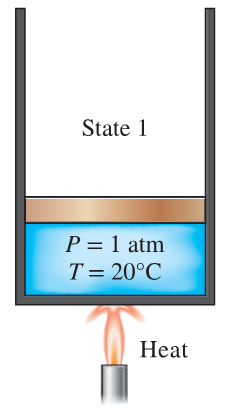
\includegraphics[width=\textwidth]{State 1.png}
\end{minipage}\\
\begin{minipage}[t]{0.7\textwidth}
\vspace{0pt}
In state 2, enough heat has been added to the water until it reaches the boiling point (100$^\circ$C at 1 atm). At this point, the water is still liquid, but any additional heat will cause it to start vaporizing, and we call this state a
\begin{itemize}
    \item \textbf{Saturated Liquid}:\\
    A liquid that is about to vaporize.
\end{itemize}
\end{minipage}
\hfill
\begin{minipage}[t]{0.2\textwidth}
\vspace{0pt}
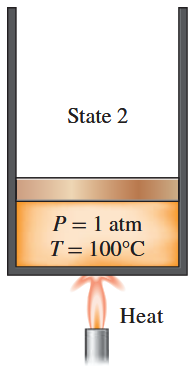
\includegraphics[width=\textwidth]{State 2.png}
\end{minipage}\\
\begin{minipage}[t]{0.7\textwidth}
\vspace{0pt}
Once boiling starts, the temperature stops rising until the liquid is completely vaporized (under constant pressure). Halfway through the boiling process, the cylinder will contain equal amounts of liquid and vapor (state 3), and we can call this state a
\begin{itemize}
    \item \textbf{Saturated Liquid–Vapor Mixture}:\\
    The phase at which liquid and vapor coexist in equilibrium. This occurs in between the start of boiling and the end of boiling.
\end{itemize}
\end{minipage}
\hspace{1.5cm}
\begin{minipage}[t]{0.35\textwidth}
\vspace{0pt}
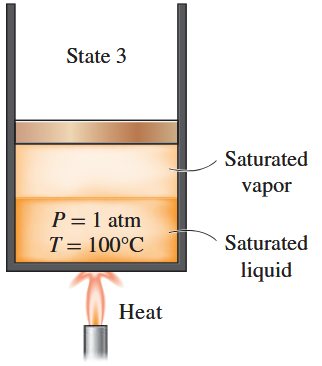
\includegraphics[width=\textwidth]{State 3.png}
\end{minipage}\\
\begin{minipage}[t]{0.7\textwidth}
\vspace{0pt}
Once vaporization is complete, the cylinder is now filled with only vapor (state 4), any heat loss will cause the vapor to start condensing back into liquid, and we call this state a
\begin{itemize}
    \item \textbf{Saturated Vapor}:\\
    A vapor that is about to condense.
\end{itemize}
\end{minipage}
\hfill
\begin{minipage}[t]{0.2\textwidth}
\vspace{0pt}
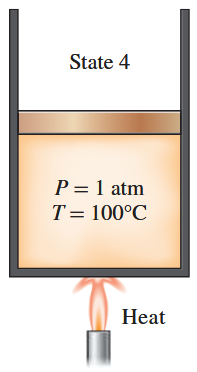
\includegraphics[width=\textwidth]{State 4.png}
\end{minipage}\\
\begin{minipage}[t]{0.7\textwidth}
\vspace{0pt}
Suppose we continue heating the vapor well beyond the boiling point (100$^\circ$C at 1 atm), even if we remove some heat, the vapor will not condense back into liquid until it reaches the boiling point again. This state is called a
\begin{itemize}
    \item \textbf{Superheated Vapor}:\\
    A vapor that is not about to condense.
\end{itemize}
\end{minipage}
\hfill
\begin{minipage}[t]{0.2\textwidth}
\vspace{0pt}
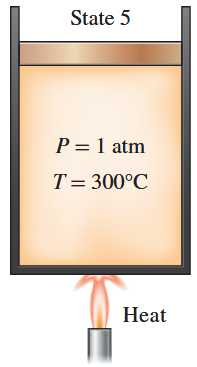
\includegraphics[width=\textwidth]{State 5.png}
\end{minipage}\\\\
These states can be visualized on the following $T-\svol$ plot. Note that if we cooled down the cylinder from state 5, keeping pressure constant, it would follow the same path back to state 1.
\begin{center}
    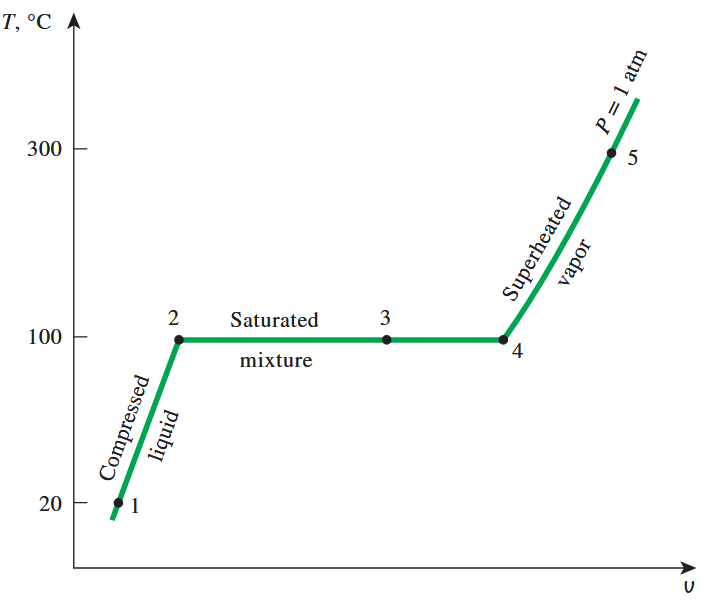
\includegraphics[width=0.7\textwidth]{Phase.png}
\end{center}
Where the plotted line represents an \textbf{isobar} (constant pressure), and the points are equilibrium states.\\\\
\textbf{Saturation Temperature and Saturation Pressure}\\
At a fixed pressure, the temperature at which a pure substance changes phase is called the \textbf{saturation temperature} $T_{sat}$, and at a fixed temperature, the pressure at which a pure substance changes phase is called the \textbf{saturation pressure} $P_{sat}$. We will be referring to the appendix tables for these values.\\\\
\textbf{Latent Heat}
\begin{itemize}
    \item \textbf{Latent Heat}: the amount of energy absorbed or released during a phase change process
    \item \textbf{Latent Heat of Vaporization} ($h_{fg}$): the amount of energy absorbed during melting or released during freezing
    \item \textbf{Latent Heat of Fusion}: the amount of energy absorbed during vaporization or released during condensation
\end{itemize}
\section*{Property Diagrams for Phase-Change Processes}
As we saw before, when a pure substance undergoes a phase change, its properties change in a specific way. We can visualize these changes using plots such as $P-\svol$, $T-\svol$, and $P-T$ diagrams.
\newpage\noindent
\underline{\textbf{$T-\svol$ Diagram}\\}
\begin{center}
    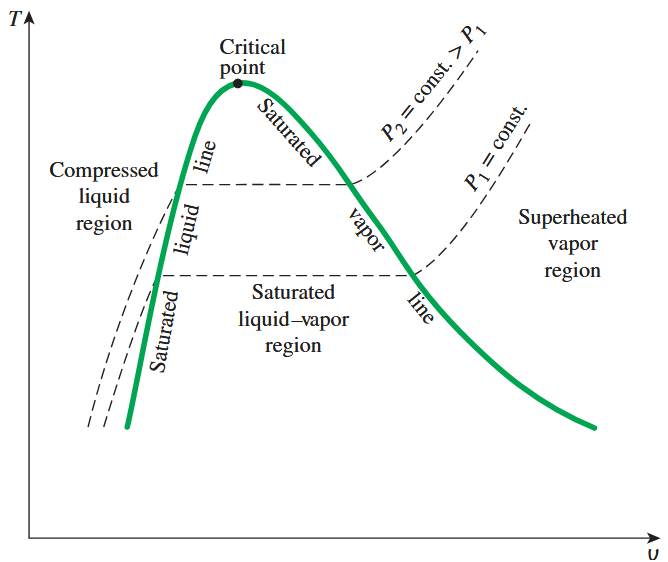
\includegraphics[width=0.7\textwidth]{TV.png}
\end{center}
The dome is called the \textbf{vapor dome} and the area under the dome represents the \textit{saturated liquid–vapor mixture} region or the \textit{wet} region. Notice that as pressure increases, the \textbf{saturation line} (horizontal line between saturated liquid and saturated vapor) becomes shorter and shorter until it eventually disappears at the \textbf{critical point}. Thus, at the critical point, the properties of the saturated liquid and saturated vapor are the same, and we cannot tell the difference between the two.\\\\
Note that the dashed lines represent \textbf{isobars} (constant pressure lines).\\\\
\begin{center}
    
\includegraphics[width=0.25\textwidth]{Chicken.jpg}
    \captionof*{figure}{A chicken}
\end{center}
\newpage\noindent
\underline{\textbf{$P-\svol$ Diagram}\\}
\begin{center}
    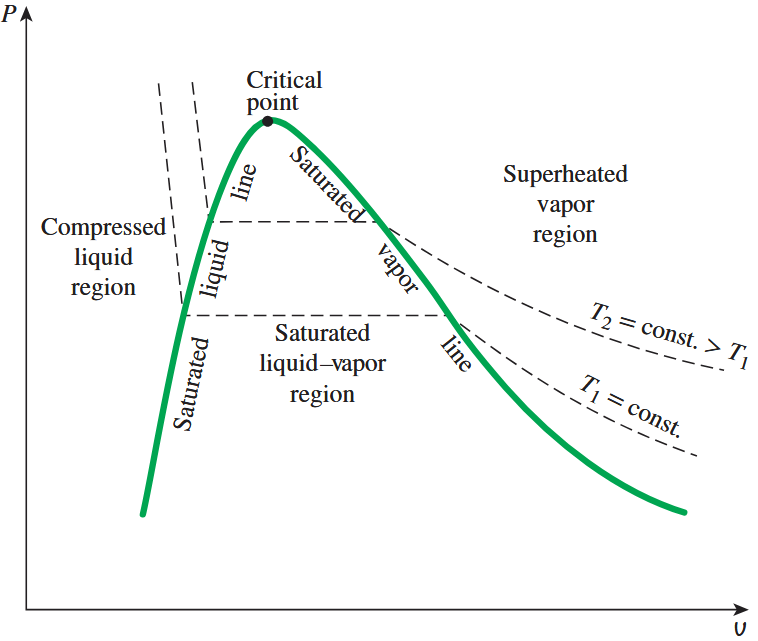
\includegraphics[width=0.7\textwidth]{PV.png}
\end{center}
Similar to a $T-\svol$ diagram, but now the dashed lines represent \textbf{isotherms} (constant temperature lines), isobars will just be horizontal lines.\\\\
\underline{\textbf{$P-T$ Diagram}\\}
\begin{center}
    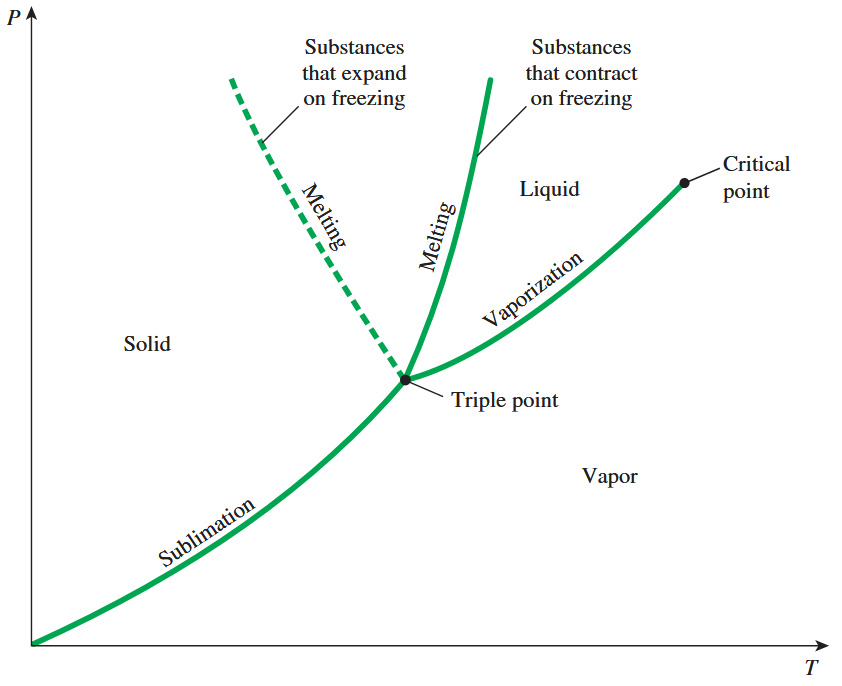
\includegraphics[width=0.7\textwidth]{PT.png}
\end{center}
The $P-T$ diagram is a more commonly known as a \textbf{phase diagram}, it shows the different phases of a substance and the conditions under which they exist.\\\\
As previously mentioned in chapter 1, all three of these diagrams are just projections of the same $P-\svol-T$ surface onto their respective planes:
\begin{center}
    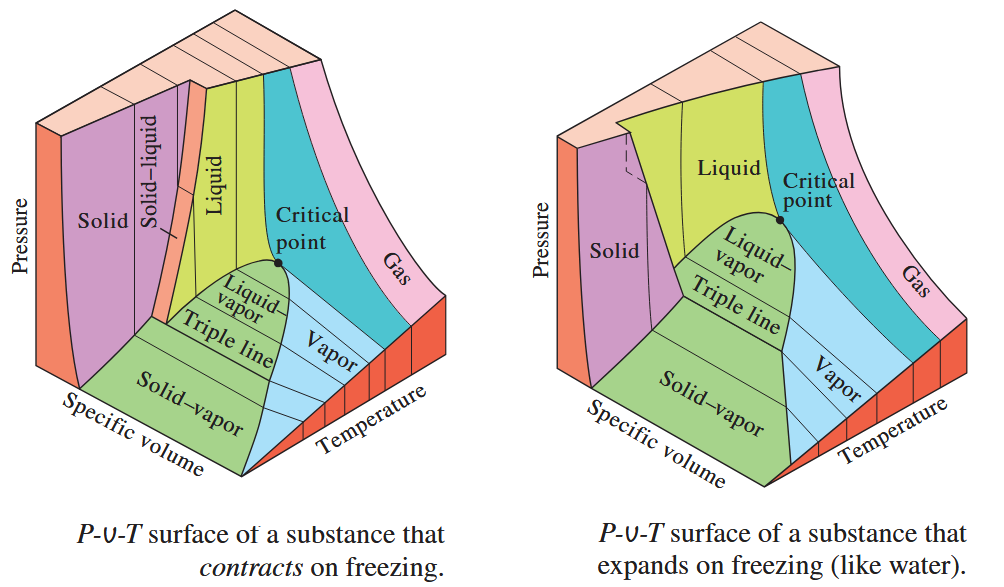
\includegraphics[width=0.8\textwidth]{PVT.png}
\end{center}
\section*{Property Tables}
Along with the visualizations of phase behavior, we have tables and values that quantify these properties. These tables will list various properties of pure substances and categorized based on each region of interest (superheated vapor, compressed liquid, and saturated mixture regions).\\\\
\textbf{Enthalpy - Revisited}\\
Like mentioned before in chapter 2, enthalpy is defined for the sake of convenience (it is a combination of internal energy and flow energy), but it saves a lot of unit conversions and math to just have it as a property in the tables.
\[h=u+P\svol\quad\text{(kJ/kg)} \quad \text{and}\quad H=U+P\vol\quad\text{(kJ)}\]
\underline{Note:} The latent heat of vaporization can be expressed in terms of enthalpy as $h_{fg} = h_g - h_f$.\\\\
\textbf{Quality in the Saturated Mixture Region}\\
In the saturated mixture region, we define the \textbf{quality} $x$ as the fraction of mixture that is vapor (by mass):
\[\boxed{x = \frac{m_\text{g}}{m_\text{g} + m_\text{f}}}\]
Where $m_g$ is the mass of the vapor and $m_f$ is the mass of the liquid.\\\\
A saturated mixture consists of saturated liquid and saturated vapor existing in equilibrium, where each phase has its own specific volume, internal energy, and enthalpy. Thus, the overall properties of the mixture can be determined as weighted averages of the corresponding saturated liquid and saturated vapor values, weighted by the quality $x$ (if there is more vapor, the properties will be closer to the saturated vapor values, and if there is more liquid, the properties will be closer to the saturated liquid values):
\begin{center}
\fbox{%
\(
\begin{aligned}
\svol_{\text{avg}} &= \svol_f + x(\svol_g - \svol_f) \quad \text{(m$^3$/kg)}\\
u_{\text{avg}}     &= u_f + x(u_g - u_f) \quad \text{(kJ/kg)}\\
h_{\text{avg}}     &= h_f + x(h_g - h_f) \quad \text{(kJ/kg)}
\end{aligned}
\)
}
\end{center}
Where the subscript $f$ refers to the saturated liquid values and the subscript $g$ refers to the saturated vapor values.\\\\
\underline{Note:} $\svol_{fg} = \svol_g - \svol_f$ is the difference in specific volume between the saturated vapor and saturated liquid, and it is also the length of the horizontal saturation line in both the $T-\svol$ and $P-\svol$ diagrams.
\begin{center}
    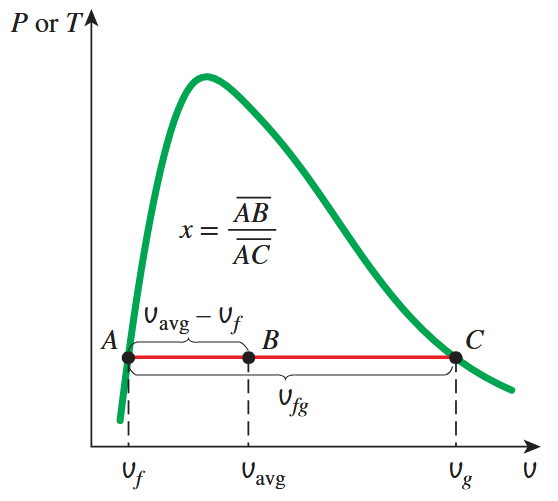
\includegraphics[width=0.6\textwidth]{Quality.png}
\end{center}
This is very similar to the concept of tie-lines in phase diagrams from materials science.\\\\
We can also find the quality of a saturated mixture if we are given the specific volume, internal energy, or enthalpy of the mixture by rearranging the above equations. For example:
\[\boxed{x = \frac{\svol_\text{avg}-\svol_\text{f}}{\svol_\text{fg}}}\]
\newpage\noindent
\textbf{How to Identify a Superheated Vapor}\\
In a saturated mixture, temperature and pressure are not independent. During phase change, any added energy is used to convert liquid into vapor rather than to increase temperature, so temperature remains fixed at the saturation value corresponding to that pressure (see before on saturation pressure/temperature). As long as both phases are present, specifying either temperature or pressure automatically determines the other.\\\\
In the superheated vapor region, the substance exists entirely as vapor, and no phase change occurs. So temperature and pressure can vary independently, and both properties must be specified to fully determine the state.\\\\
We can tell if a state is in the superheated vapor region if it satisfies any of the following conditions:
\begin{itemize}
    \item Lower pressures ($P < P_{\text{sat}}$ at a given $T$)
    \item Higher temperatures ($T > T_{\text{sat}}$ at a given $P$)
    \item Higher specific volumes ($\svol > \svol_g$ at a given $P$ or $T$)
    \item Higher internal energies ($u > u_g$ at a given $P$ or $T$)
    \item Higher enthalpies ($h > h_g$ at a given $P$ or $T$)
\end{itemize}
Generally, these conditions compare the state properties to the corresponding saturation properties at the same temperature or pressure. If the state has properties that exceed those of the saturated vapor, it is in the superheated region.\\\\
\underline{Note:} The opposite conditions (compared to saturated liquid conditions) would indicate a compressed liquid state, and if the state properties match the saturated liquid or saturated vapor properties, then it is in the saturated liquid or saturated vapor state, respectively.\\\\
\textbf{Compressed Liquid Approximation}\\
There aren't as many data points for compressed liquids in the tables. However, in the compressed liquid region, the specific volume, internal energy, and enthalpy of the substance are very close to those of the saturated liquid at the same temperature. Therefore, we \textit{approximate the properties of a compressed liquid by using the saturated liquid properties at the same temperature.}\\\\
\textbf{Reference State + Values}\\
The values of internal energy, enthalpy, and entropy are not measured directly and are given relative to a reference state. The reference state for water is taken at the saturated liquid state at 0.01$^\circ$C where $u=0$, $h=0$, and $s=0$.\\\\
Sometimes different tables use different references states, but the math will work out as long as we are consistent with the table we are using. 








\end{document}